\section{User Interface}
This section features designs for the different areas of the system. Wireframes of each screens are provided, giving a general impression of what the screen will look like once implemented. It should be remembered, of course, that design, particularly that of a visual nature, is an iterative process, and, as such, the final product may differ, perhaps wildly, from the screens featured here.

\subsection{Input Methods}
The school plans to use the system on both desktop PCs and tablets. As such, the system will support input through both a mouse and keyboard, as well as a touchscreen. For the quiz creator, input boxes will be used to allow users to enter information like the quiz title, questions, answers, etc. Buttons will also be used, allowing users to perform actions. In the quiz playing section, buttons will be used, as all the information needed for the quiz will have already been entered.

\subsection{Colours and Typography}
As revealed through interviews conducted with staff, the school is placing a great deal of emphasis on the design of the application. As such, a unique approach to the interface will be taken, one that resonates with the new found focus on houses within the school.

\subsubsection{Typography}
In order to make the system yet more appealing and approachable, the font ``Dosis'' will be used throughout. As show by the example below, Dosis is a friendly font, one that invites the user to perform actions. This is in line with the objectives for the system, and will make the system suitable for all ages in the school. An example can be seen in the next subsection.

\subsubsection{Colours}
Each house has their own colour, and this colour will be used to theme all elements of the interface, depending on the house that a student is logged in as. The colour mappings are as follows:

\begin{itemize}[leftmargin=*]
  \item \dosis{\textcolor{specialblue}{Acton (Blue)}}
  \item \dosis{\textcolor{specialorange}{Baxter (Orange)}}
  \item \dosis{\textcolor{specialturquoise}{Clive (Turqoise)}}
  \item \dosis{\textcolor{specialpurple}{Darwin (Purple)}}
  \item \dosis{\textcolor{specialred}{Houseman (Red)}}
  \item \dosis{\textcolor{specialyellow}{Webb (Yellow)}}
\end{itemize}

In order to ensure that each user sees a subtedly different design, even if they are in the same house, the colours will be randomised. For example, a user in Acton might see buttons in a light blue and drop down boxes in a dark blue, whilst another user in Acton would see slightly darker or lighter shades. In order to make the system more appealing to use, the luminosity of each colour will be locked to a certain brightness.

\subsection{Login Screen}
\begin{figure}[h!]
  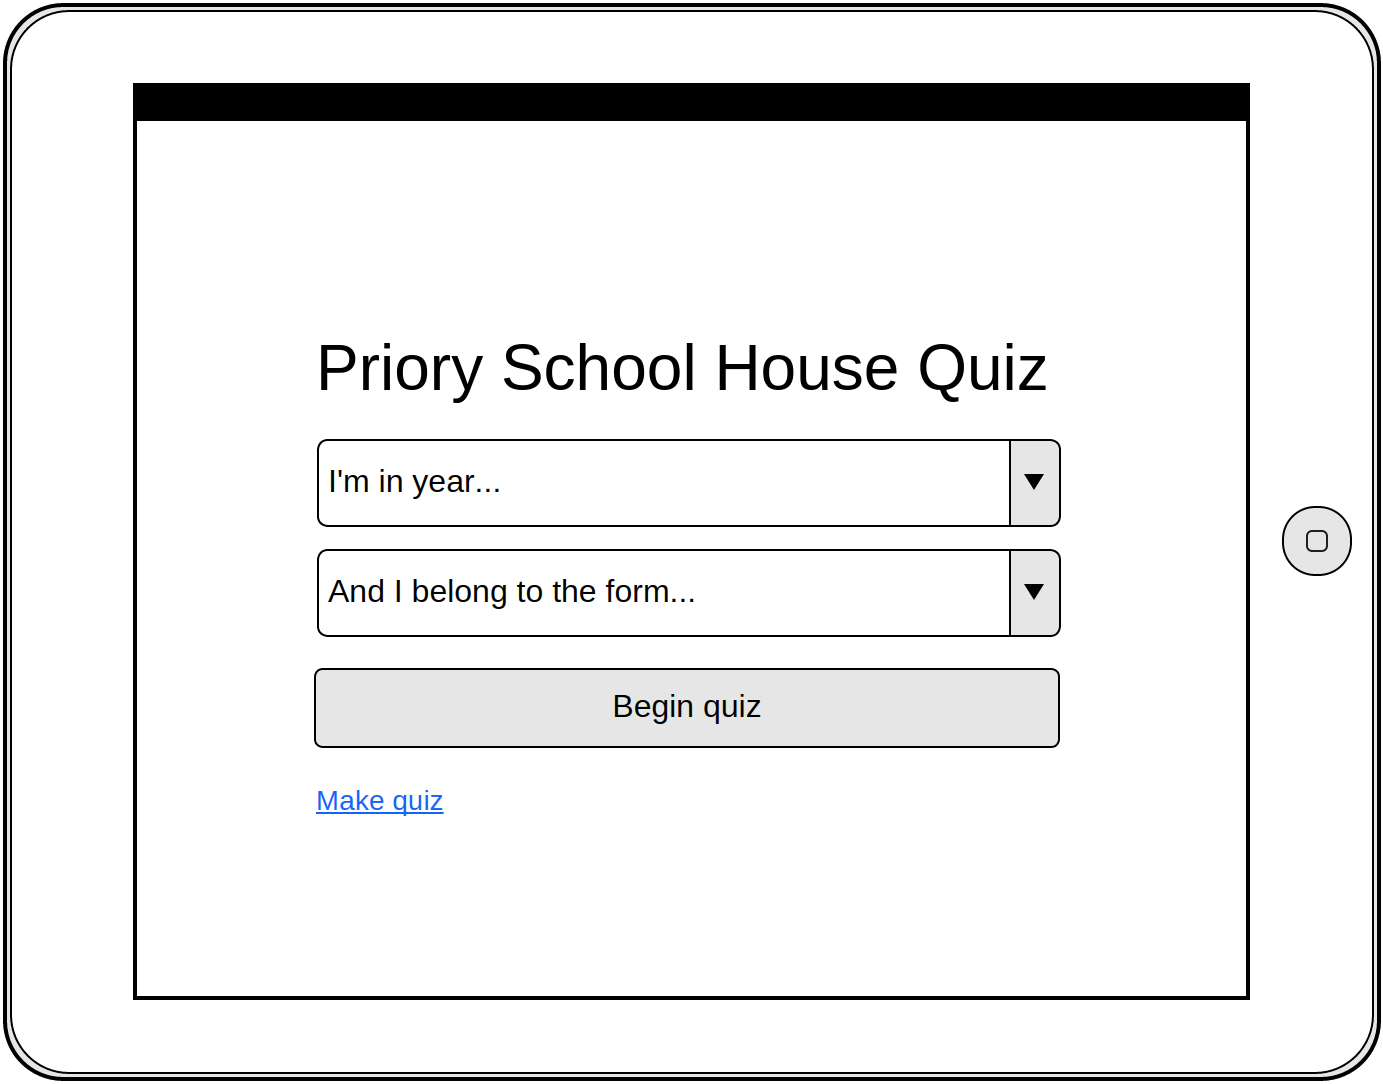
\includegraphics[scale=0.24]{design/login}
\end{figure}

Due to the way the school names individual form groups, a simplified approach to the login form can be used. Two drop down boxes will be used, one for the year - containing the items 7, 8, 9, 10 and 11 - and one for the house - Acton, Baxter, Clive, Darwin, Houseman, Webb. By doing this, any combination of form group can be computed. Interviews with students revealed that they would not be likely to pose as a member of another form group, so no authentication is needed - students need simply enter their year group and house, and then press the ``Begin quiz'' button. If a senior member of staff needs to create a quiz, clicking the link will bring them to a password prompt, in order to prevent errant students making a quiz themselves. Because the user will not have chosen their house, house colours will not be available. Instead, the colours of all the houses will feature, with the interface elements changing every few seconds to the next house.

\subsection{Countdown Screen}
\begin{figure}[h!]
  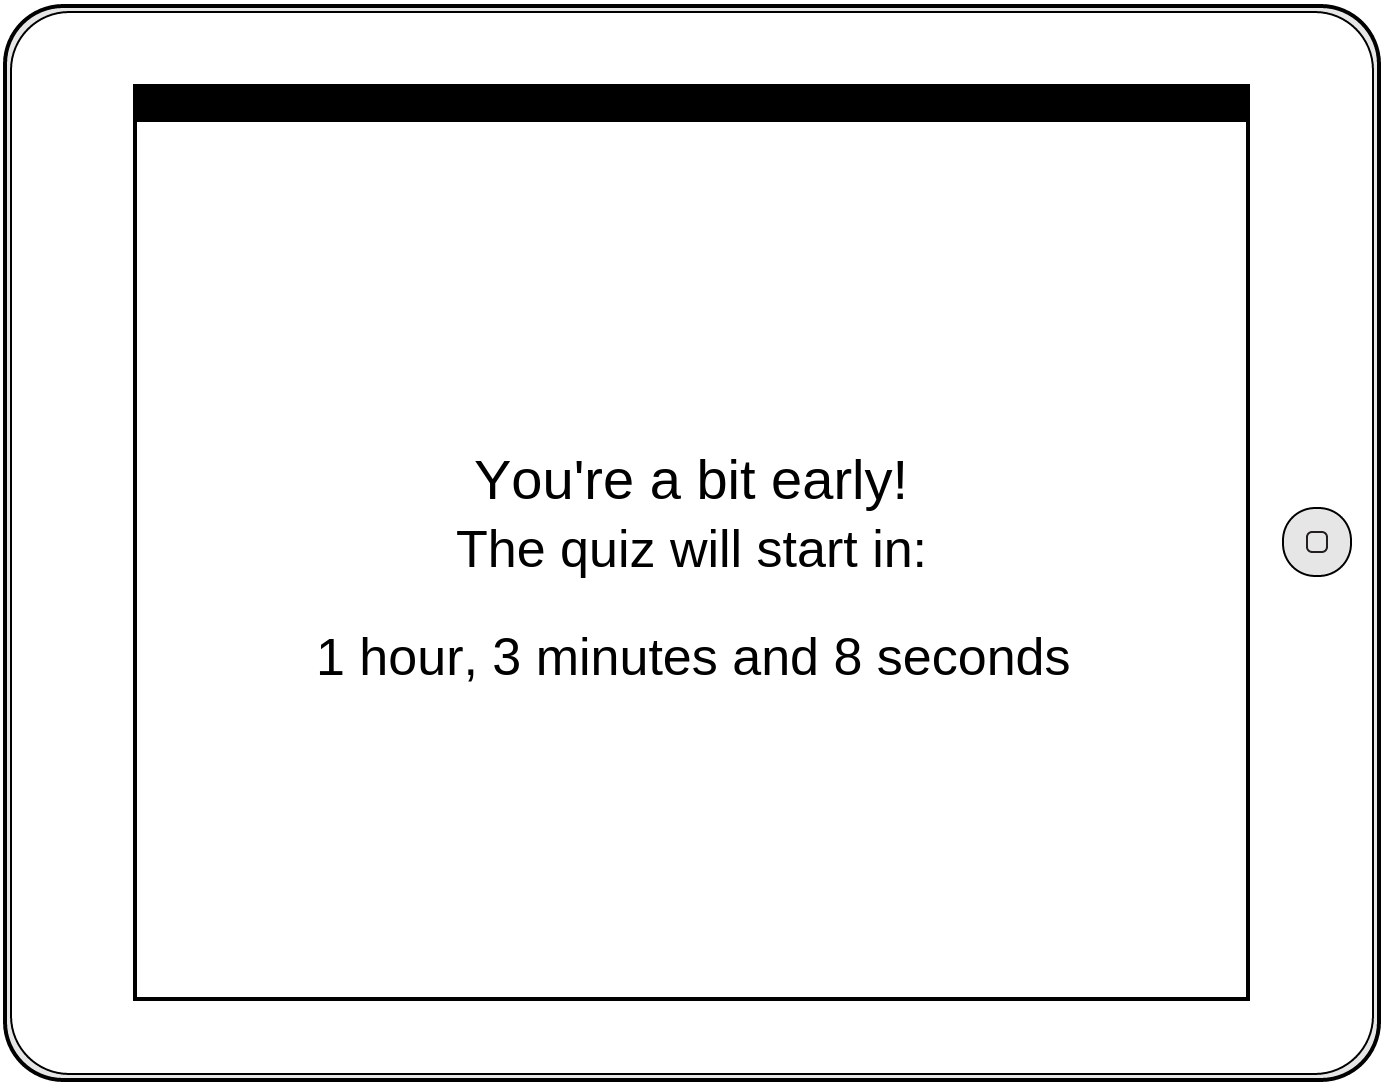
\includegraphics[scale=0.24]{design/countdown}
\end{figure}

In the event that a student logs onto the system and a quiz is yet to start, this screen will be displayed, informing them how long they have to wait. The countdown timer will display the time till the next scheduled quiz in hours, minutes and seconds, and will update accordingly.

\clearpage

\subsection{Quiz Creation Screen}
\begin{figure}[h!]
  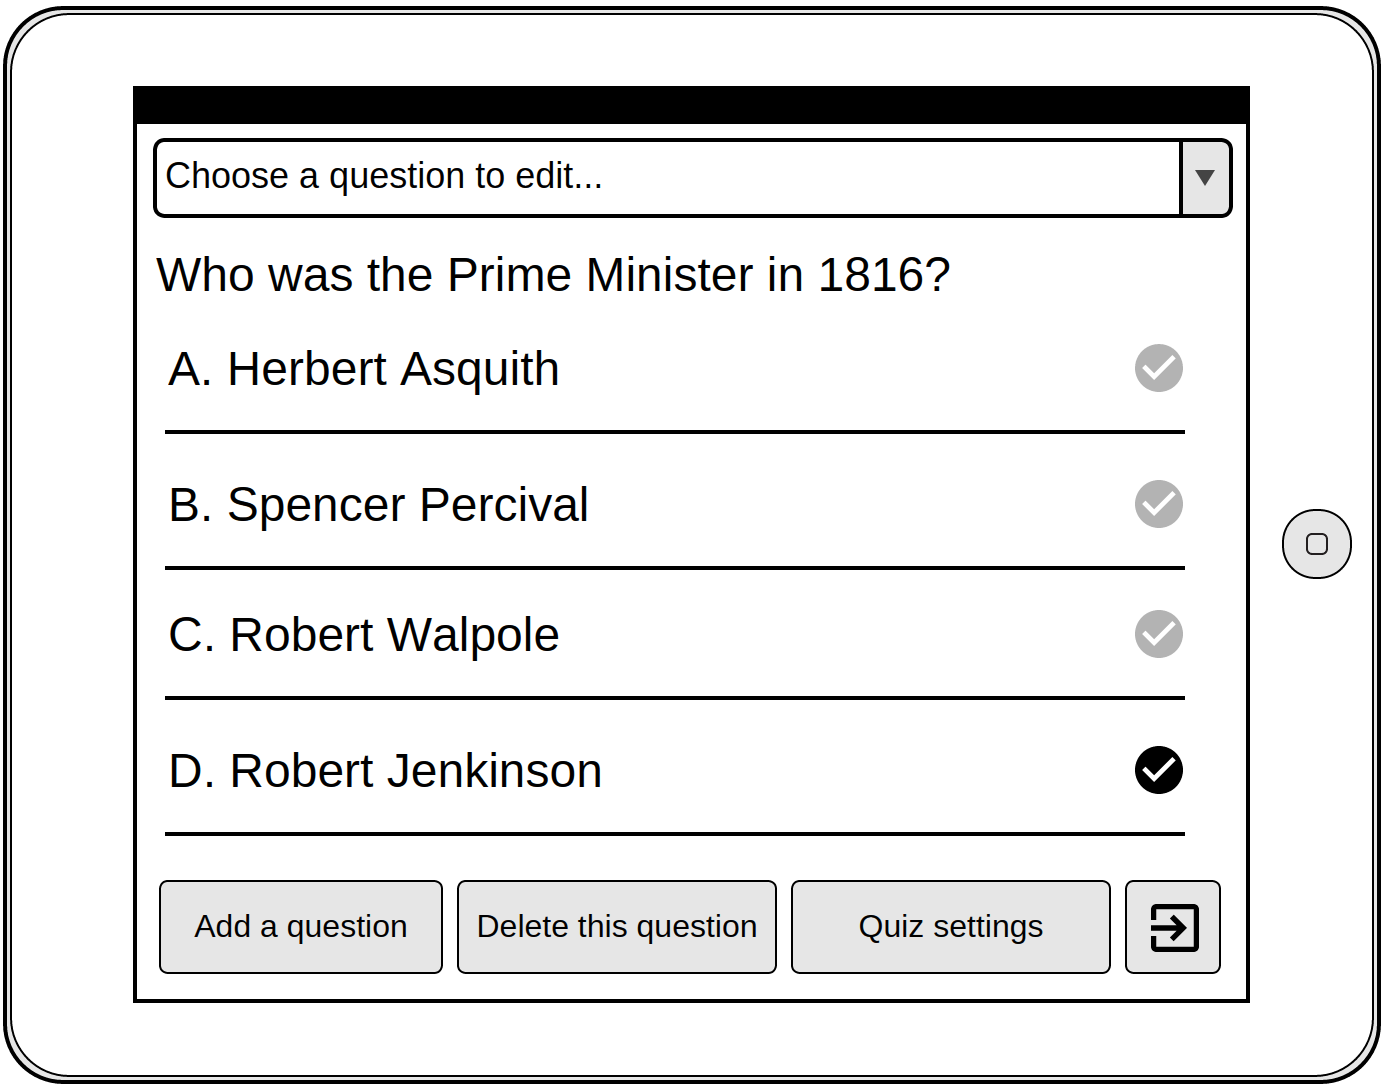
\includegraphics[scale=0.24]{design/quiz_maker}
\end{figure}

This screen will be available to members of staff, and will allow them to create quizzes for the students to consume. A dropdown box at the top will allow staff to switch between questions in the quiz, enabling them to easily go back and make changes. The question title is displayed just below this; tapping on it will allow staff to make changes. Just below this will be the four possible answers to the question (each question must have four answers), which staff can add in appropriately. By the side of each possible answer will be a complication to allow staff to mark an answer as correct; only one answer can be correct at a time. Below this are a series of buttons, granting the ability to add or delete questions, modify the quiz settings, such as the title; and leave the quiz maker.

\clearpage

\subsection{Play Quiz Screen}
\begin{figure}[h!]
  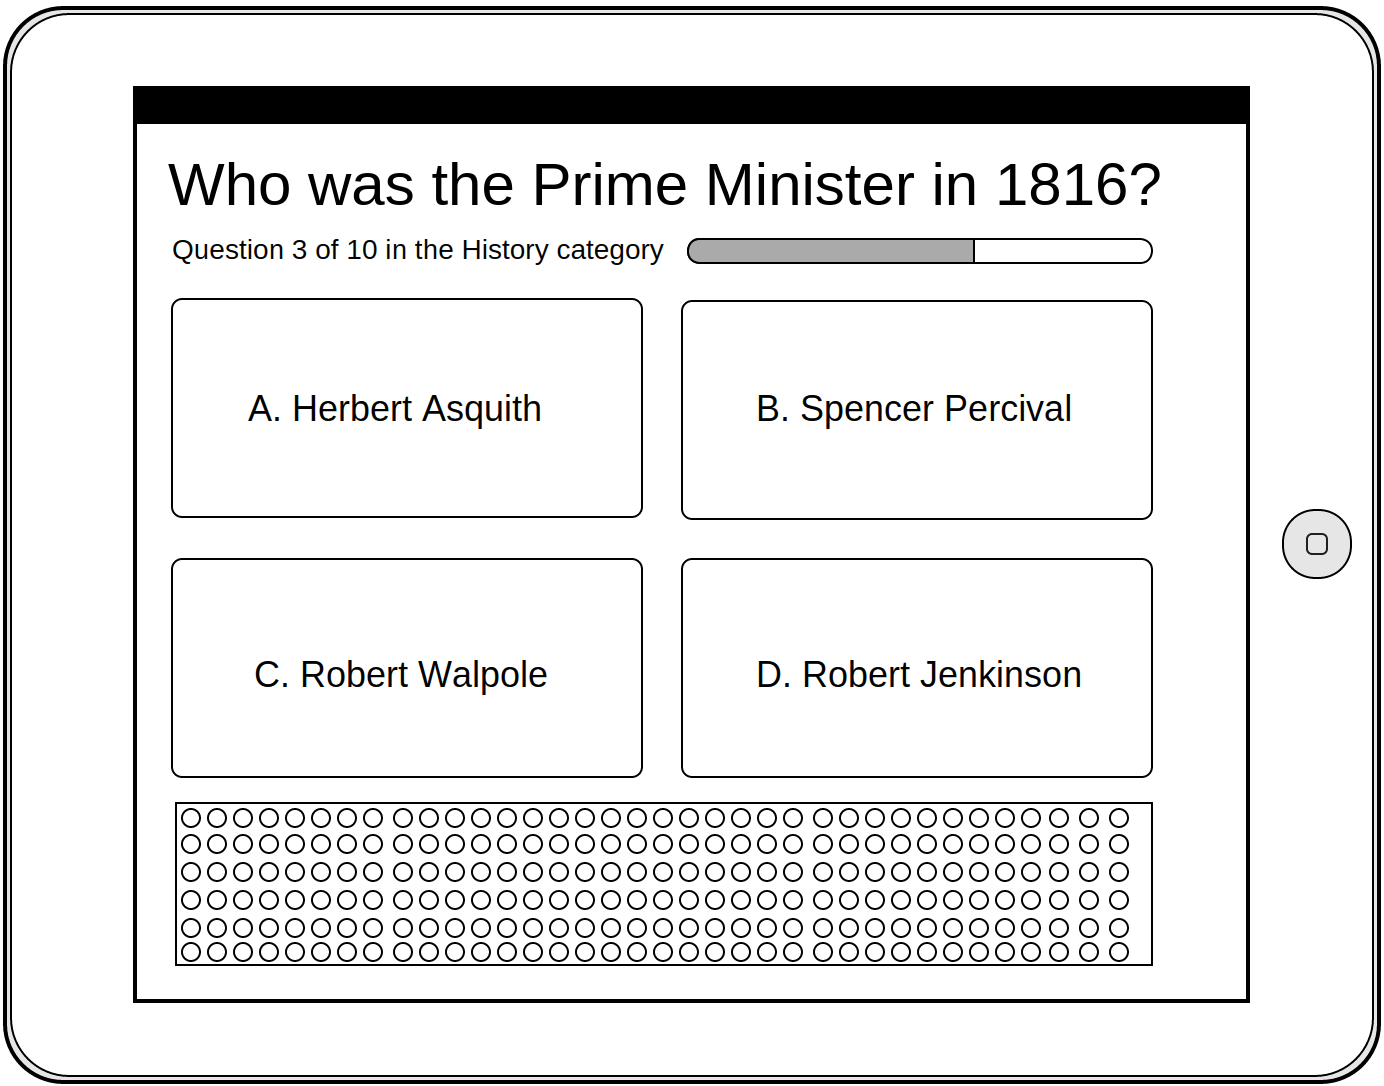
\includegraphics[scale=0.24]{design/quiz_play}
\end{figure}

This is the main screen of the system, and the one that users will spend the most time on - the actual quiz interface. At the top, the current question will be displayed, enabling users to gain a clear impression of what they are meant to be answering. Below, the current position in the quiz, including the current category, will be shown, letting users see how much longer the quiz will last. Next to this wil be a progress bar acting as the question timer - it will fill up for each question, providing a visual representation of how long the user has left to answer the question. Below this will be the actual question answers; to select one, the user need simply tap on it. Just below this will be a button to activate ``peek mode''. This will activate the view so exalted by Nick Bucknall in the interviews, displaying a real time overlay on the question options of how other people in the school are voting. Pressing the button again will turn this view off, though it will be activated automatically once the user chooses an answer.
